\documentclass[tikz,border=8pt]{standalone}
% Shared look for every TikZ diagram. Load with % Shared look for every TikZ diagram. Load with % Shared look for every TikZ diagram. Load with \input{../../tools/tikz-style.tex}
\usepackage[T1]{fontenc}
\usepackage{lmodern}
\renewcommand{\sfdefault}{lmr}  % diagrams use the same serif as the text
\usetikzlibrary{arrows.meta, positioning, shapes.geometric, calc, fit, backgrounds}
\definecolor{cblue}{HTML}{4C78A8}
\definecolor{corange}{HTML}{F58518}
\definecolor{cgreen}{HTML}{54A24B}
\definecolor{cred}{HTML}{E45756}
\definecolor{cpurple}{HTML}{B279A2}
\definecolor{cgrey}{HTML}{6B6B6B}
\tikzset{
  every picture/.style={font=\sffamily, line width=1.2pt},
  box/.style={draw=#1, fill=#1!12, rounded corners=4pt, align=center, inner sep=7pt, minimum height=1.1cm},
  box/.default=cgrey,
  arrow/.style={-{Stealth[length=3mm]}, draw=cgrey, line width=1.4pt},
  title/.style={font=\sffamily\bfseries\Large},
  note/.style={font=\sffamily\small, text=cgrey, align=center},
}
\AtBeginDocument{\hyphenpenalty=10000 \exhyphenpenalty=10000}

\usepackage[T1]{fontenc}
\usepackage{lmodern}
\renewcommand{\sfdefault}{lmr}  % diagrams use the same serif as the text
\usetikzlibrary{arrows.meta, positioning, shapes.geometric, calc, fit, backgrounds}
\definecolor{cblue}{HTML}{4C78A8}
\definecolor{corange}{HTML}{F58518}
\definecolor{cgreen}{HTML}{54A24B}
\definecolor{cred}{HTML}{E45756}
\definecolor{cpurple}{HTML}{B279A2}
\definecolor{cgrey}{HTML}{6B6B6B}
\tikzset{
  every picture/.style={font=\sffamily, line width=1.2pt},
  box/.style={draw=#1, fill=#1!12, rounded corners=4pt, align=center, inner sep=7pt, minimum height=1.1cm},
  box/.default=cgrey,
  arrow/.style={-{Stealth[length=3mm]}, draw=cgrey, line width=1.4pt},
  title/.style={font=\sffamily\bfseries\Large},
  note/.style={font=\sffamily\small, text=cgrey, align=center},
}
\AtBeginDocument{\hyphenpenalty=10000 \exhyphenpenalty=10000}

\usepackage[T1]{fontenc}
\usepackage{lmodern}
\renewcommand{\sfdefault}{lmr}  % diagrams use the same serif as the text
\usetikzlibrary{arrows.meta, positioning, shapes.geometric, calc, fit, backgrounds}
\definecolor{cblue}{HTML}{4C78A8}
\definecolor{corange}{HTML}{F58518}
\definecolor{cgreen}{HTML}{54A24B}
\definecolor{cred}{HTML}{E45756}
\definecolor{cpurple}{HTML}{B279A2}
\definecolor{cgrey}{HTML}{6B6B6B}
\tikzset{
  every picture/.style={font=\sffamily, line width=1.2pt},
  box/.style={draw=#1, fill=#1!12, rounded corners=4pt, align=center, inner sep=7pt, minimum height=1.1cm},
  box/.default=cgrey,
  arrow/.style={-{Stealth[length=3mm]}, draw=cgrey, line width=1.4pt},
  title/.style={font=\sffamily\bfseries\Large},
  note/.style={font=\sffamily\small, text=cgrey, align=center},
}
\AtBeginDocument{\hyphenpenalty=10000 \exhyphenpenalty=10000}

\begin{document}
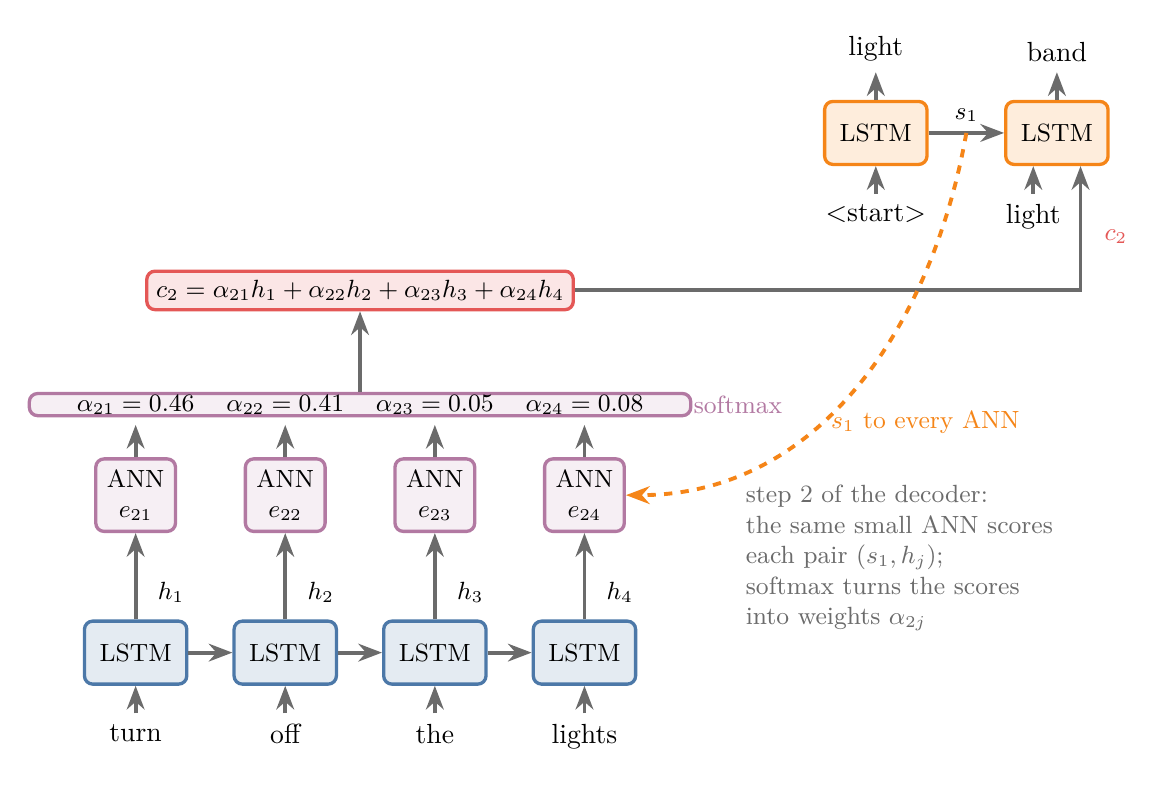
\begin{tikzpicture}[cell/.style={draw=#1, fill=#1!15, minimum width=1.3cm, minimum height=0.8cm, rounded corners=3pt, font=\sffamily\small},
  word/.style={font=\sffamily}, op/.style={draw=cpurple, fill=cpurple!12, rounded corners=3pt, align=center, font=\sffamily\small, inner sep=4pt}]
  % encoder
  \foreach \w [count=\j] in {turn, off, the, lights} {
    \node[cell=cblue] (e\j) at (1.9*\j, 0) {LSTM};
    \node[word, below=0.35cm of e\j] (x\j) {\w};
    \draw[arrow] (x\j) -- (e\j);
    \node[font=\sffamily\small, above=0.08cm of e\j, xshift=0.45cm] (hl\j) {$h_\j$};
  }
  \foreach \i/\j in {1/2, 2/3, 3/4} \draw[arrow] (e\i) -- (e\j);
  % alignment model, one per encoder state (same weights)
  \foreach \j/\a in {1/0.46, 2/0.41, 3/0.05, 4/0.08} {
    \node[op] (f\j) at (1.9*\j, 2.0) {ANN\\$e_{2\j}$};
    \draw[arrow] (e\j.north) -- (f\j.south);
    \node[font=\sffamily\small] (a\j) at (1.9*\j, 3.15) {$\alpha_{2\j} = \a$};
    \draw[arrow] (f\j) -- (a\j);
  }
  \node[op, minimum width=8.4cm] (sm) at (4.75, 3.15) {};
  \node[font=\sffamily\small, text=cpurple] at (9.55, 3.15) {softmax};
  \foreach \j/\a in {1/0.46, 2/0.41, 3/0.05, 4/0.08} \node[font=\sffamily\small] at (1.9*\j, 3.15) {$\alpha_{2\j} = \a$};
  % weighted sum
  \node[draw=cred, fill=cred!15, rounded corners=3pt, font=\sffamily\small, align=center] (c) at (4.75, 4.6)
    {$c_2 = \alpha_{21}h_1 + \alpha_{22}h_2 + \alpha_{23}h_3 + \alpha_{24}h_4$};
  \draw[arrow] (sm) -- (c);
  % decoder
  \node[cell=corange] (d1) at (11.3, 6.6) {LSTM};
  \node[cell=corange] (d2) at (13.6, 6.6) {LSTM};
  \node[word, below=0.35cm of d1] (y0) {$<$start$>$};
  \node[word, below=0.35cm of d2, xshift=-0.3cm] (y1) {light};
  \draw[arrow] (y0) -- (d1); \draw[arrow] (y1) -- (y1 |- d2.south);
  \draw[arrow] (d1) -- node[above, font=\sffamily\small] {$s_1$} (d2);
  \node[word, above=0.35cm of d1] (o1) {light};
  \node[word, above=0.35cm of d2] (o2) {band};
  \draw[arrow] (d1) -- (o1); \draw[arrow] (d2) -- (o2);
  \draw[arrow] (c.east) -| ($(d2.south)+(0.3,-1.25)$) -- ($(d2.south)+(0.3,0)$);
  \node[font=\sffamily\small, text=cred] at ($(d2.south)+(0.75,-0.9)$) {$c_2$};
  % s1 feeds every ANN
  \draw[arrow, draw=corange, dashed] ($(d1.east)!0.5!(d2.west)$) to[out=-100, in=0] node[pos=0.6, right, font=\sffamily\small, text=corange] {$s_1$ to every ANN} (f4.east);
  \node[note, align=left] at (11.6, 1.2) {step 2 of the decoder:\\the same small ANN scores\\each pair $(s_1, h_j)$;\\softmax turns the scores\\into weights $\alpha_{2j}$};
\end{tikzpicture}
\end{document}
